\section{CMOS MAPS}

    %%%%%%%%%%%%%%%%%%%%%%%%%%%%%%%%%%%%%%%%
    %%  Slide 2: <CMOS MAPS concept>  %%
    %%%%%%%%%%%%%%%%%%%%%%%%%%%%%%%%%%%%%%%%
    \begin{frame}
        \frametitle{CMOS Monolitich Active Pixel Sensors}
        %forse anche la terza parentesi con minore circa 100 um
        \begin{columns}
            \column{0.4\textwidth}
                \vspace*{-0.6cm}
                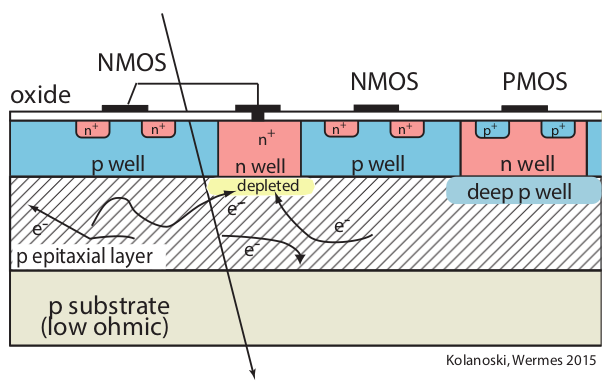
\includegraphics[width=1.15\linewidth]{figures/Pixel_detectors/MAPS_scheme.png}
            \column{0.6\textwidth}  
                \begin{tikzpicture}[overlay]
                    \draw[decorate,decoration={brace}]
                        (0,-0.6) -- node[xshift=2pt,anchor=west] {$\lesssim$\SI{5}{\um} electronics}(0,-1.15);
                \medskip
                    \draw[decorate,decoration={brace}]
                        (0,-1.25) -- node[xshift=2pt,anchor=west] {$\lesssim$\SI{50}{\um} sensor}(0,-1.9);
                \end{tikzpicture}
                \bigskip
                \begin{equation*}
                    \hspace{80pt} d \propto \sqrt{\rho V}
                \end{equation*}   
                \begin{equation*}
                    %\hspace{75pt} ENC^2 \propto \frac{4}{3} \frac{kT}{g_m} \frac{C_D ^2}{\tau_{sh}}
                    \hspace{80pt} ENC^2 \propto C_D ^2
                \end{equation*}  
                \begin{equation*}
                    %\hspace{75pt} \tau \propto \frac{1}{g_m}\frac{C_D}{C_f}
                    \hspace{80pt} \tau \propto C_D
                \end{equation*}  
                \begin{equation*}
                    \hspace{80pt} Q_{MIP}\propto d \sim 80 e^-/\si{\um}
                \end{equation*}  
            \end{columns}   
        \medskip 
        \begin{itemize}
            \item An epitaxial layer with doping few order of magnitude smaller than the subtrate is introduced below the surface
            \item Electronics is low resistivity while sensor needs high $\rho$, special technologies for the sensor have been implemented. 
            \item High resistivity allows for depleted epi-layer DMAPS
            \item If not completed depleted charge is collected by diffusion
            \item MAPS have a very low capacity 
        \end{itemize}
    \end{frame} 



    %%%%%%%%%%%%%%%%%%%%%%%%%%%%%%%%%%%%%%%%
    %%  Slide 3: <Sensors types>  %%
    %%%%%%%%%%%%%%%%%%%%%%%%%%%%%%%%%%%%%%%%
    \begin{frame}
        \frametitle{Sensor types}
            \begin{itemize}
                \item \textbf{Large fill factor} ($\sim$100-200 \si{fF}) or \textbf{small fill factor} ($<$\SI{5}{fF}), depending on the deep p-well structures
            \end{itemize}
            %\centering
            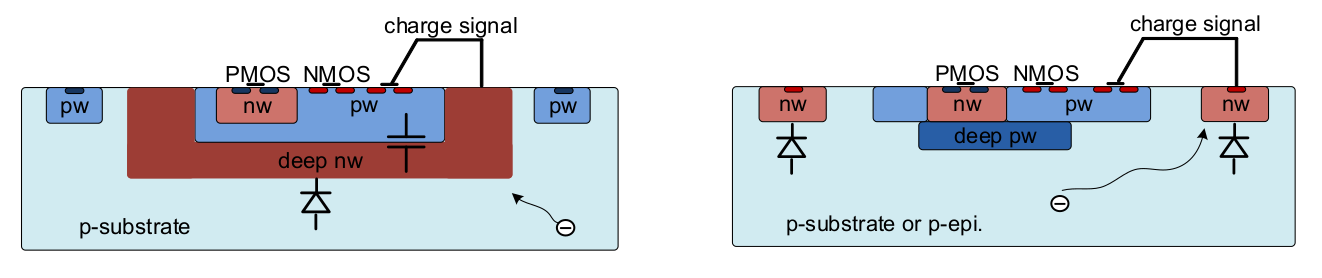
\includegraphics[width=1.05\linewidth]{figures/Pixel_detectors/large_small_sensor_scheme.png}\\
            \begin{columns}
                \column{0.5\textwidth}  
                    %\centering
                    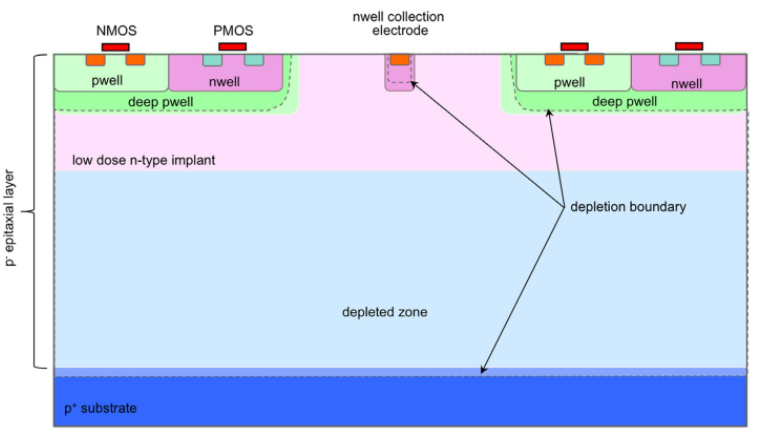
\includegraphics[width=1.1\linewidth]{figures/Pixel_detectors/ALPIDE_after_PM.png}
                \column{0.5\textwidth}  
                    \begin{itemize}
                        \item \textbf{Process modification} with a low dose planar implant. \\
                        whose main investigator is ALICE\\
                        %Advantage: no need of change in the sensor and circuit layout
                    \end{itemize} 
            \end{columns}

            \end{frame} 

    %%%%%%%%%%%%%%%%%%%%%%%%%%%%%%%%%%%%%%%%
    %%  Slide 1: <READOUT>  %%
    %%%%%%%%%%%%%%%%%%%%%%%%%%%%%%%%%%%%%%%%
    \begin{frame}
        \frametitle{Front end}
            \begin{columns}
                \column{0.7\textwidth}  
                \textbf{Pixel area economy} and dimension of components are extremely relevant. \\
                MAPS usage allowed by miniaturization of components: starting from \SI{600}{nm} down to 120-180{nm} CMOS process.
                \column{0.4\textwidth}  
                    \begin{figure}[h!]
                        \vspace*{-0.85cm}
                        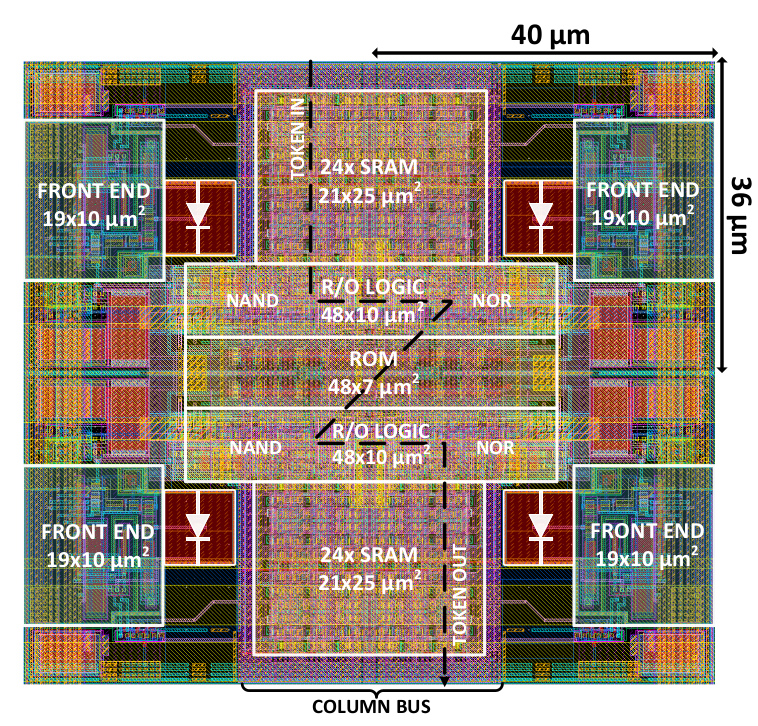
\includegraphics[width=1.05\linewidth]{figures/Monopix1/Monopix1_2x2pixelsgroup.png}
                    \end{figure}
            \end{columns}
        \begin{itemize}
            \item Analog or digital output
            \item Triggered or triggerless
            \item Buffer on pixel to store more than one hit data
            \item Rolling shut or sparsified (data push) readout, for example column drain is one of the most popular.
        \end{itemize}
 
    \end{frame} 


    %%%%%%%%%%%%%%%%%%%%%%%%%%%%%%%%%%%%%%%%
    %%  Slide 1: <ALICE>  %%
    %%%%%%%%%%%%%%%%%%%%%%%%%%%%%%%%%%%%%%%%
    \begin{frame}
        \frametitle{ALPIDE - ALice PIxel DEtector}
        ALICE ITS2 upgraded in 2019-20\\
        \smallskip
        The \textbf{sensor} uses high resistivity p-type epi-layer, TowerJazz in \SI{0.18}{\um}. It is the first large area $\sim$\SI{10}{m\squared} MAPS detector with sparsified readout.
        Many MAPS have an \textbf{ALPIDE-based Front End} (i.e. TJ-Monopix1, ARCADIA)
        \begin{columns}
            \column{0.35\textwidth}  
                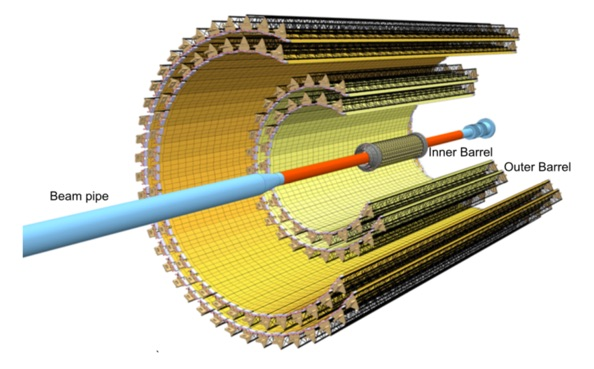
\includegraphics[width=1.3\linewidth]{figures/pixel_detectors_usage/alice.png}
            \column{0.6\textwidth}
            \begin{itemize}
                \item position measurement $\sim$\SI{5}{\um} (pixel dimension 27$\times$29\si{\um\squared})
                \item X$_0$ reduced from 1.14\% to 0.3\% per layer
                \item efficiency of track reconstruction improves of a factor 6 for low momentum particles with $p_T \sim$\SI{0.1}{GeV/c}
            \end{itemize}
        \end{columns}
        %ALPIDE is under test for several other HEP detectors (i.e. Belle2) and applications and 
    \end{frame} 